% Created 2023-10-11 Wed 13:54
% Intended LaTeX compiler: pdflatex
\documentclass[presentation, t]{beamer}
\usepackage[utf8]{inputenc}
\usepackage[T1]{fontenc}
\usepackage{fontspec}
\usepackage{xcolor}
\usepackage{hyperref}
\usepackage{cleveref}
% features: (acronym underline par-sep .pifont beamer image table .missing-koma checkbox)
\newcommand{\acr}[1]{\protect\textls*[110]{\scshape #1}}
\newcommand{\acrs}{\protect\scalebox{.91}[.84]{\hspace{0.15ex}s}}
\usepackage[normalem]{ulem}
\setlength{\parskip}{\baselineskip}
\setlength{\parindent}{0pt}

\usepackage{pifont}
\usepackage{graphicx}
\usepackage{longtable}
\usepackage{booktabs}
\usepackage{scrextend}
\usepackage{amssymb} % provides \square
\newcommand{\checkboxUnchecked}{$\square$}
\newcommand{\checkboxTransitive}{\rlap{\raisebox{-0.1ex}{\hspace{0.35ex}\Large\textbf -}}$\square$}
\newcommand{\checkboxChecked}{\rlap{\raisebox{0.2ex}{\hspace{0.35ex}\scriptsize \ding{52}}}$\square$}

% end features

%% make document follow Emacs theme

\definecolor{obg}{HTML}{2E3440}
\definecolor{ofg}{HTML}{ECEFF4}

% heading colours
\definecolor{documentTitle}{HTML}{81A1C1}
\definecolor{documentInfo}{HTML}{81A1C1}
\definecolor{level1}{HTML}{81A1C1}
\definecolor{level2}{HTML}{B48EAD}
\definecolor{level3}{HTML}{5D80AE}
\definecolor{level4}{HTML}{a0b8d0}
\definecolor{level5}{HTML}{c6aac1}
\definecolor{level6}{HTML}{c0d0e0}
\definecolor{level7}{HTML}{d9c6d6}
\definecolor{level8}{HTML}{e5ecf2}

% textual elements

\definecolor{link}{HTML}{81A1C1}
\colorlet{url}{link}
\definecolor{cite}{HTML}{88C0D0}
\definecolor{itemlabel}{HTML}{81A1C1}
\definecolor{code}{HTML}{B48EAD}
\definecolor{verbatim}{HTML}{A3BE8C}

\DeclareTextFontCommand{\texttt}{\color{code}\ttfamily}

\let\oldverb\verb
\def\verb{\bgroup\color{verbatim}\oldverb}
\makeatletter
\let\verb@oldegroup\verb@egroup
\def\verb@egroup{\verb@oldegroup\egroup}
\makeatother

% beamer

\definecolor{builtin}{HTML}{81A1C1}
\definecolor{varname}{HTML}{D8DEE9}

\NewCommandCopy{\oldusetheme}{\usetheme}
\renewcommand*{\usetheme}[2][]{\oldusetheme[#1]{#2}
  \setbeamercolor{title separator}{fg=documentTitle}
  \setbeamercolor{progress bar}{fg=documentTitle}
  \setbeamercolor{progress bar in head/foot}{fg=documentTitle}
  \setbeamercolor{progress bar in section page}{fg=documentTitle}

  \setbeamercolor{normal text}{fg=ofg, bg=obg}
  \setbeamercolor{alerted text}{fg=varname}
  \setbeamercolor*{item}{fg=itemlabel}
  \setbeamercolor{block title}{fg=level3, bg=}
}

\usepackage{etoolbox}
\makeatletter
\patchcmd{\beamer@section}{%
  \edef\insertsectionhead{\noexpand\hyperlink{Navigation\the\c@page}{\unexpanded{#1}}}}{%
  \edef\insertsectionhead{\begingroup\noexpand\hypersetup{hidelinks}\noexpand\hyperlink{Navigation\the\c@page}{\unexpanded{#1}}\endgroup}}
\makeatother

% code blocks

\definecolor{codebackground}{HTML}{373E4C}
\colorlet{EFD}{ofg}
\definecolor{codeborder}{HTML}{404654}

%% end customisations

\usetheme[progressbar=foot]{metropolis}
\author{Ellis Kenyő}
\date{\today}
\title{Org-a-nice Your Life In Emacs}
\subtitle{\footnotesize https://orgmode.org/}
\titlegraphic{
\includegraphics[height=1.5cm]{org-mode-unicorn.png}}
\usepackage{pgfpages}
\usepackage{graphicx}
\setbeameroption{show notes on second screen=right}
\setbeamertemplate{note page}{\insertnote\par}
\newcommand{\btVFill}{\vskip0pt plus 1filll}
\colorlet{greenyblue}{blue!70!green}
\colorlet{blueygreen}{blue!40!green}
\providecolor{link}{named}{greenyblue}
\providecolor{cite}{named}{blueygreen}
\hypersetup{
  pdfauthor={Ellis Kenyő},
  pdftitle={Org-a-nice Your Life In Emacs},
  pdfkeywords={},
  pdfsubject={},
  pdfcreator={Emacs 30.0.50 (Org mode 9.7)},
  pdflang={English},
  breaklinks=true,
  colorlinks=true,
  linkcolor=,
  urlcolor=link,
  citecolor=cite
}
\urlstyle{same}

% Setup for code blocks [1/2]

\usepackage{fvextra}

\fvset{%
  commandchars=\\\{\},
  highlightcolor=white!95!black!80!blue,
  breaklines=true,
  breaksymbol=\color{white!60!black}\tiny\ensuremath{\hookrightarrow}}

% Make line numbers smaller and grey.
\renewcommand\theFancyVerbLine{\footnotesize\color{black!40!white}\arabic{FancyVerbLine}}

\usepackage{xcolor}

% In case engrave-faces-latex-gen-preamble has not been run.
\providecolor{EfD}{HTML}{f7f7f7}
\providecolor{EFD}{HTML}{28292e}

% Define a Code environment to prettily wrap the fontified code.
\usepackage[breakable,xparse]{tcolorbox}
\DeclareTColorBox[]{Code}{o}%
{colback=EfD!98!EFD, colframe=EfD!95!EFD,
  fontupper=\footnotesize\setlength{\fboxsep}{0pt},
  colupper=EFD,
  IfNoValueTF={#1}%
  {boxsep=2pt, arc=2.5pt, outer arc=2.5pt,
    boxrule=0.5pt, left=2pt}%
  {boxsep=2.5pt, arc=0pt, outer arc=0pt,
    boxrule=0pt, leftrule=1.5pt, left=0.5pt},
  right=2pt, top=1pt, bottom=0.5pt,
  breakable}

% Support listings with captions
\usepackage{float}
\floatstyle{plain}
\newfloat{listing}{htbp}{lst}
\newcommand{\listingsname}{Listing}
\floatname{listing}{\listingsname}
\newcommand{\listoflistingsname}{List of Listings}
\providecommand{\listoflistings}{\listof{listing}{\listoflistingsname}}


% Setup for code blocks [2/2]: syntax highlighting colors

\newcommand\efstrut{\vrule height 2.1ex depth 0.8ex width 0pt}
\definecolor{EFD}{HTML}{ECEFF4}
\definecolor{EfD}{HTML}{2E3440}
\newcommand{\EFD}[1]{\textcolor{EFD}{#1}} % default
\newcommand{\EFvp}[1]{#1} % variable-pitch
\definecolor{EFh}{HTML}{4C566A}
\newcommand{\EFh}[1]{\textcolor{EFh}{#1}} % shadow
\definecolor{EFsc}{HTML}{A3BE8C}
\newcommand{\EFsc}[1]{\textcolor{EFsc}{#1}} % success
\definecolor{EFw}{HTML}{EBCB8B}
\newcommand{\EFw}[1]{\textcolor{EFw}{#1}} % warning
\definecolor{EFe}{HTML}{BF616A}
\newcommand{\EFe}[1]{\textcolor{EFe}{#1}} % error
\definecolor{EFl}{HTML}{81A1C1}
\newcommand{\EFl}[1]{\textcolor{EFl}{\textbf{#1}}} % link
\definecolor{EFlv}{HTML}{ee82ee}
\newcommand{\EFlv}[1]{\textcolor{EFlv}{\textbf{#1}}} % link-visited
\definecolor{EFhi}{HTML}{191C25}
\definecolor{Efhi}{HTML}{81A1C1}
\newcommand{\EFhi}[1]{\colorbox{Efhi}{\efstrut{}\textcolor{EFhi}{#1}}} % highlight
\definecolor{EFc}{HTML}{6f7787}
\newcommand{\EFc}[1]{\textcolor{EFc}{#1}} % font-lock-comment-face
\definecolor{EFcd}{HTML}{6f7787}
\newcommand{\EFcd}[1]{\textcolor{EFcd}{#1}} % font-lock-comment-delimiter-face
\definecolor{EFs}{HTML}{A3BE8C}
\newcommand{\EFs}[1]{\textcolor{EFs}{#1}} % font-lock-string-face
\definecolor{EFd}{HTML}{78808f}
\newcommand{\EFd}[1]{\textcolor{EFd}{#1}} % font-lock-doc-face
\definecolor{EFm}{HTML}{81A1C1}
\newcommand{\EFm}[1]{\textcolor{EFm}{#1}} % font-lock-doc-markup-face
\definecolor{EFk}{HTML}{81A1C1}
\newcommand{\EFk}[1]{\textcolor{EFk}{#1}} % font-lock-keyword-face
\definecolor{EFb}{HTML}{81A1C1}
\newcommand{\EFb}[1]{\textcolor{EFb}{#1}} % font-lock-builtin-face
\definecolor{EFf}{HTML}{88C0D0}
\newcommand{\EFf}[1]{\textcolor{EFf}{#1}} % font-lock-function-name-face
\definecolor{EFv}{HTML}{D8DEE9}
\newcommand{\EFv}[1]{\textcolor{EFv}{#1}} % font-lock-variable-name-face
\definecolor{EFt}{HTML}{8FBCBB}
\newcommand{\EFt}[1]{\textcolor{EFt}{#1}} % font-lock-type-face
\definecolor{EFo}{HTML}{81A1C1}
\newcommand{\EFo}[1]{\textcolor{EFo}{#1}} % font-lock-constant-face
\definecolor{EFwr}{HTML}{EBCB8B}
\newcommand{\EFwr}[1]{\textcolor{EFwr}{#1}} % font-lock-warning-face
\definecolor{EFnc}{HTML}{81A1C1}
\newcommand{\EFnc}[1]{\textcolor{EFnc}{\textbf{#1}}} % font-lock-negation-char-face
\definecolor{EFpp}{HTML}{81A1C1}
\newcommand{\EFpp}[1]{\textcolor{EFpp}{\textbf{#1}}} % font-lock-preprocessor-face
\definecolor{EFrc}{HTML}{81A1C1}
\newcommand{\EFrc}[1]{\textcolor{EFrc}{\textbf{#1}}} % font-lock-regexp-grouping-construct
\definecolor{EFrb}{HTML}{81A1C1}
\newcommand{\EFrb}[1]{\textcolor{EFrb}{\textbf{#1}}} % font-lock-regexp-grouping-backslash
\definecolor{Efob}{HTML}{373E4C}
\newcommand{\EFob}[1]{\colorbox{Efob}{\efstrut{}#1}} % org-block
\definecolor{EFobb}{HTML}{6f7787}
\definecolor{Efobb}{HTML}{373E4C}
\newcommand{\EFobb}[1]{\colorbox{Efobb}{\efstrut{}\textcolor{EFobb}{#1}}} % org-block-begin-line
\definecolor{EFobe}{HTML}{6f7787}
\definecolor{Efobe}{HTML}{373E4C}
\newcommand{\EFobe}[1]{\colorbox{Efobe}{\efstrut{}\textcolor{EFobe}{#1}}} % org-block-end-line
\definecolor{EFOa}{HTML}{81A1C1}
\newcommand{\EFOa}[1]{\textcolor{EFOa}{\textbf{#1}}} % outline-1
\definecolor{EFOb}{HTML}{B48EAD}
\newcommand{\EFOb}[1]{\textcolor{EFOb}{\textbf{#1}}} % outline-2
\definecolor{EFOc}{HTML}{5D80AE}
\newcommand{\EFOc}[1]{\textcolor{EFOc}{\textbf{#1}}} % outline-3
\definecolor{EFOd}{HTML}{a0b8d0}
\newcommand{\EFOd}[1]{\textcolor{EFOd}{\textbf{#1}}} % outline-4
\definecolor{EFOe}{HTML}{c6aac1}
\newcommand{\EFOe}[1]{\textcolor{EFOe}{\textbf{#1}}} % outline-5
\definecolor{EFOf}{HTML}{c0d0e0}
\newcommand{\EFOf}[1]{\textcolor{EFOf}{\textbf{#1}}} % outline-6
\definecolor{EFOg}{HTML}{d9c6d6}
\newcommand{\EFOg}[1]{\textcolor{EFOg}{\textbf{#1}}} % outline-7
\definecolor{EFOh}{HTML}{e5ecf2}
\newcommand{\EFOh}[1]{\textcolor{EFOh}{\textbf{#1}}} % outline-8
\definecolor{EFhn}{HTML}{B48EAD}
\newcommand{\EFhn}[1]{\textcolor{EFhn}{\textbf{#1}}} % highlight-numbers-number
\definecolor{EFhq}{HTML}{81A1C1}
\newcommand{\EFhq}[1]{\textcolor{EFhq}{#1}} % highlight-quoted-quote
\definecolor{EFhs}{HTML}{8FBCBB}
\newcommand{\EFhs}[1]{\textcolor{EFhs}{#1}} % highlight-quoted-symbol
\definecolor{EFrda}{HTML}{81A1C1}
\newcommand{\EFrda}[1]{\textcolor{EFrda}{#1}} % rainbow-delimiters-depth-1-face
\definecolor{EFrdb}{HTML}{B48EAD}
\newcommand{\EFrdb}[1]{\textcolor{EFrdb}{#1}} % rainbow-delimiters-depth-2-face
\definecolor{EFrdc}{HTML}{A3BE8C}
\newcommand{\EFrdc}[1]{\textcolor{EFrdc}{#1}} % rainbow-delimiters-depth-3-face
\definecolor{EFrdd}{HTML}{5D80AE}
\newcommand{\EFrdd}[1]{\textcolor{EFrdd}{#1}} % rainbow-delimiters-depth-4-face
\definecolor{EFrde}{HTML}{8FBCBB}
\newcommand{\EFrde}[1]{\textcolor{EFrde}{#1}} % rainbow-delimiters-depth-5-face
\definecolor{EFrdf}{HTML}{81A1C1}
\newcommand{\EFrdf}[1]{\textcolor{EFrdf}{#1}} % rainbow-delimiters-depth-6-face
\definecolor{EFrdg}{HTML}{B48EAD}
\newcommand{\EFrdg}[1]{\textcolor{EFrdg}{#1}} % rainbow-delimiters-depth-7-face
\definecolor{EFrdh}{HTML}{A3BE8C}
\newcommand{\EFrdh}[1]{\textcolor{EFrdh}{#1}} % rainbow-delimiters-depth-8-face
\definecolor{EFrdi}{HTML}{5D80AE}
\newcommand{\EFrdi}[1]{\textcolor{EFrdi}{#1}} % rainbow-delimiters-depth-9-face
\definecolor{EFany}{HTML}{EBCB8B}
\definecolor{Efany}{HTML}{EBCB8B}
\newcommand{\EFany}[1]{\colorbox{Efany}{\efstrut{}\textcolor{EFany}{#1}}} % ansi-color-yellow
\definecolor{EFanr}{HTML}{BF616A}
\definecolor{Efanr}{HTML}{BF616A}
\newcommand{\EFanr}[1]{\colorbox{Efanr}{\efstrut{}\textcolor{EFanr}{#1}}} % ansi-color-red
\definecolor{EFanb}{HTML}{2E3440}
\newcommand{\EFanb}[1]{\textcolor{EFanb}{#1}} % ansi-color-black
\definecolor{EFang}{HTML}{A3BE8C}
\definecolor{Efang}{HTML}{A3BE8C}
\newcommand{\EFang}[1]{\colorbox{Efang}{\efstrut{}\textcolor{EFang}{#1}}} % ansi-color-green
\definecolor{EFanB}{HTML}{81A1C1}
\definecolor{EfanB}{HTML}{81A1C1}
\newcommand{\EFanB}[1]{\colorbox{EfanB}{\efstrut{}\textcolor{EFanB}{#1}}} % ansi-color-blue
\definecolor{EFanc}{HTML}{88C0D0}
\definecolor{Efanc}{HTML}{88C0D0}
\newcommand{\EFanc}[1]{\colorbox{Efanc}{\efstrut{}\textcolor{EFanc}{#1}}} % ansi-color-cyan
\definecolor{Efanw}{HTML}{ECEFF4}
\newcommand{\EFanw}[1]{\colorbox{Efanw}{\efstrut{}#1}} % ansi-color-white
\definecolor{EFanm}{HTML}{B48EAD}
\definecolor{Efanm}{HTML}{B48EAD}
\newcommand{\EFanm}[1]{\colorbox{Efanm}{\efstrut{}\textcolor{EFanm}{#1}}} % ansi-color-magenta
\definecolor{EFANy}{HTML}{edd29c}
\definecolor{EfANy}{HTML}{edd29c}
\newcommand{\EFANy}[1]{\colorbox{EfANy}{\efstrut{}\textcolor{EFANy}{#1}}} % ansi-color-bright-yellow
\definecolor{EFANr}{HTML}{c87880}
\definecolor{EfANr}{HTML}{c87880}
\newcommand{\EFANr}[1]{\colorbox{EfANr}{\efstrut{}\textcolor{EFANr}{#1}}} % ansi-color-bright-red
\definecolor{EFANb}{HTML}{191C25}
\definecolor{EfANb}{HTML}{2C333F}
\newcommand{\EFANb}[1]{\colorbox{EfANb}{\efstrut{}\textcolor{EFANb}{#1}}} % ansi-color-bright-black
\definecolor{EFANg}{HTML}{b0c79d}
\definecolor{EfANg}{HTML}{b0c79d}
\newcommand{\EFANg}[1]{\colorbox{EfANg}{\efstrut{}\textcolor{EFANg}{#1}}} % ansi-color-bright-green
\definecolor{EFANB}{HTML}{93afca}
\definecolor{EfANB}{HTML}{93afca}
\newcommand{\EFANB}[1]{\colorbox{EfANB}{\efstrut{}\textcolor{EFANB}{#1}}} % ansi-color-bright-blue
\definecolor{EFANc}{HTML}{99c9d7}
\definecolor{EfANc}{HTML}{99c9d7}
\newcommand{\EFANc}[1]{\colorbox{EfANc}{\efstrut{}\textcolor{EFANc}{#1}}} % ansi-color-bright-cyan
\definecolor{EFANw}{HTML}{F0F4FC}
\definecolor{EfANw}{HTML}{F0F4FC}
\newcommand{\EFANw}[1]{\colorbox{EfANw}{\efstrut{}\textcolor{EFANw}{#1}}} % ansi-color-bright-white
\definecolor{EFANm}{HTML}{bf9eb9}
\definecolor{EfANm}{HTML}{bf9eb9}
\newcommand{\EFANm}[1]{\colorbox{EfANm}{\efstrut{}\textcolor{EFANm}{#1}}} % ansi-color-bright-magenta
\begin{document}

\maketitle
\note{
\tiny

Welcome everyone to my org-mode talk. I've noticed recently that there's still a
surprising amount of Emacs users who haven't yet tried out or even heard of what
I consider to be one of Emacs' big so-called ``killer apps'' that truly
differentiate it from other similar systems. I'm also undersold on asciidoc both
to read in-editor, read on github and write, of which I think org-mode is a much
better fit.

In this talk I hope to go over why it's so powerful and what exactly it can be used for.}
\section{What is Org-Mode?}
\label{sec:orgf9c98ea}
\begin{frame}[label={sec:orgc6ba473}]{ORGanizing and tracking everything in your life}
\bigskip
\begin{itemize}
\item Written by Carsten Dominik
\item Used in various domains by \href{https://orgmode.org/worg/org-people.html}{various people}
\item Note taking, agenda, document export; to name a few
\end{itemize}

\btVFill

\begin{quote}
A scientist's take on planning, note-taking, documentation and publishing using plain-text files

-- Prof. Carsten Dominik
\end{quote}
\end{frame}
\note{
\tiny

So as the name suggests; org-mode is about ORGanizing and tracking everything in your life. And as all good things are; this time it's from the comfort of Emacs. Written by a Professor called Carsten Dominik as an attempt to group together all his notes and improve his ability to capture, catalogue and index those notes; it has since evolved to have many fingers in many pies in terms of the breadth of domains and users.

Some of the functionality now encompassed by org-mode that I intend to touch on in this talk include:

\begin{itemize}
\item Note-taking
\item Agenda/time-tracking
\item Code blocks/execution
\item Document export
\end{itemize}

I also intend to touch on the wider ecosystem of org-mode and finally some example, more complex use cases; as time permits.

Included on the slide is a link to a small snippet of users, including a farmer, a mountaineer and even someone who is completely blind.}
\begin{frame}[label={sec:org2594ec1}]{What \emph{is} an org document?}
\bigskip
 \begin{center}
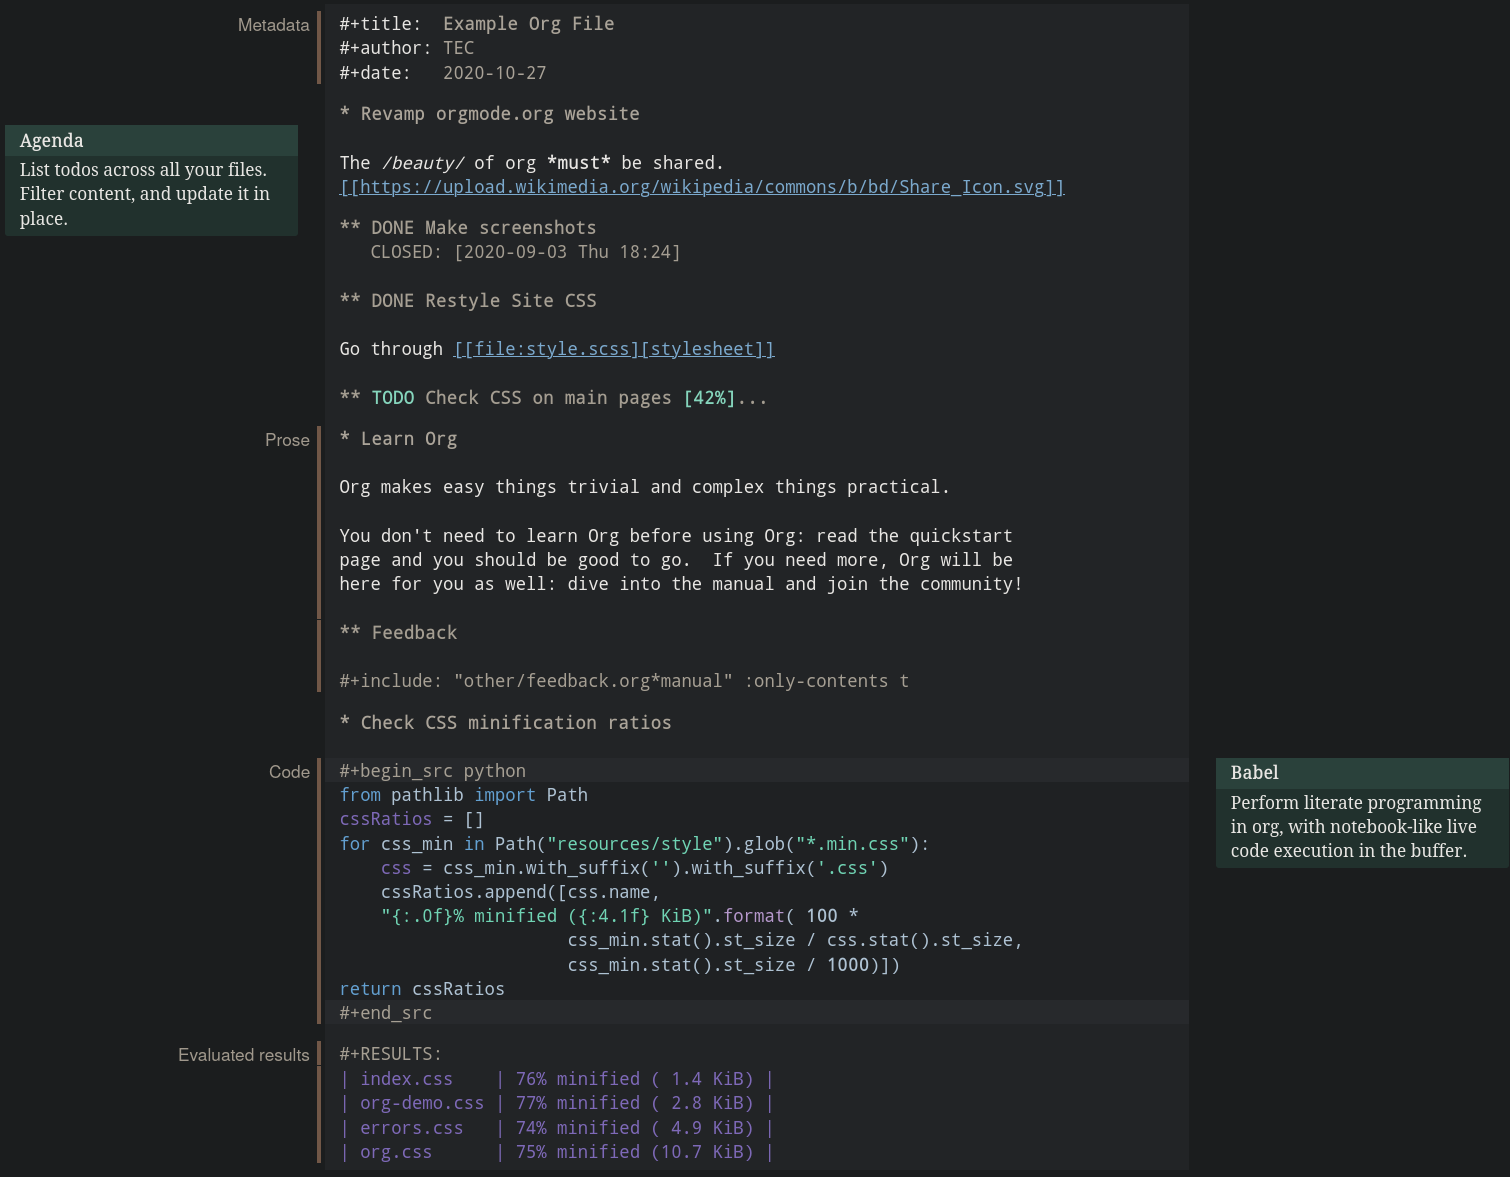
\includegraphics[width=.9\linewidth]{org-demo.png}
\end{center}
 Source: \url{https://orgmode.org/}
\end{frame}
\note{
\tiny

The image here is a demo from the org-mode website showcasing a number of org features. We'll go over what everything here means shortly in more detail, but at the end of the day it's just a plain text format.

Other packages have been written for neovim and vscode, so the majority of things here should be applicable to them too (maybe not babel and export, which we'll touch on later).

The following explanations are intended to be terse so we can get to the larger features of org, so as with everything here I encourage you to review the manual pages or ask questions at the end if something isn't clear.}
\section{Time to go deeper}
\label{sec:orgc520d71}
\begin{frame}[label={sec:org94f687e},fragile]{Headings}
 \begin{Code}
\begin{Verbatim}
\color{EFD}\textcolor[HTML]{0000ff}{*} \textcolor[HTML]{4C566A}{\textbf{DONE}} \textcolor[HTML]{4C566A}{Make screenshots}
   \textcolor[HTML]{78808f}{CLOSED:} \textcolor[HTML]{EBCB8B}{[2020-09-03 Thu 18:24]}

\textcolor[HTML]{0000ff}{*} \textcolor[HTML]{4C566A}{\textbf{DONE}} \textcolor[HTML]{4C566A}{Restyle Site CSS}
Go through \textcolor[HTML]{ff8e00}{\textbf{[[file:style.scss][stylesheet]]}}

\textcolor[HTML]{0000ff}{*} \textcolor[HTML]{A3BE8C}{\textbf{TODO}} \textcolor[HTML]{0000ff}{Check CSS on main pages} \textcolor[HTML]{A3BE8C}{\textbf{[42\%]}}
\textcolor[HTML]{81A1C1}{-} \textcolor[HTML]{4C566A}{[X]} \textcolor[HTML]{4C566A}{Index page}
\textcolor[HTML]{81A1C1}{-} \textcolor[HTML]{4C566A}{[X]} \textcolor[HTML]{4C566A}{Quickstart}
\textcolor[HTML]{81A1C1}{-} [ ] Features
\textcolor[HTML]{81A1C1}{-} [ ] Releases
\textcolor[HTML]{81A1C1}{-} \textcolor[HTML]{4C566A}{[X]} \textcolor[HTML]{4C566A}{Install}
\textcolor[HTML]{81A1C1}{-} [ ] Manual
\textcolor[HTML]{81A1C1}{-} [ ] Contribute
\end{Verbatim}
\end{Code}
\end{frame}
\note{
\tiny

Here we have a header; denoted by \texttt{*}. This can be as deep as needed, Emacs has 8 faces by default but anything past 8 it just cycles through the faces. Some of these headings also exhibit agenda properties; with the \texttt{TODO} and \texttt{DONE} keywords. These are defined in a variable called \texttt{org-todo-keywords} and denote various stages of task completion, used for the agenda we'll talk about later.

You'll also notice on the green \texttt{TODO} entry there's a percentage at the end, that denotes how many child tasks are marked as \texttt{DONE}. As items are marked off, this progress updates automatically.

Headings are the ``main'' kind of entity in a document, as the whole document is a hierarchy. If you specify no headers, everything is at the same level. But as you add them, all children then belong to a particular heading.

Useful shortcuts are included for moving headings around (including all children), promoting/demoting headings (by that I mean increasing or decreasing the nesting level) and even refiling headings (by that I mean moving them to headings in other documents)}
\begin{frame}[label={sec:org9ec6b8f},fragile]{Markup}
 - \uline{\_underline\_} *

\begin{Code}
\begin{Verbatim}
\color{EFD}\textcolor[HTML]{81A1C1}{-} /\textit{italics}/
\textcolor[HTML]{81A1C1}{-} *\textbf{bold}*
\textcolor[HTML]{81A1C1}{-} +\sout{strike-through}+
\textcolor[HTML]{81A1C1}{-} =\textcolor[HTML]{A3BE8C}{code}= and \char126{}\textcolor[HTML]{D08770}{verbatim}\char126{}
\textcolor[HTML]{81A1C1}{-} \textcolor[HTML]{81A1C1}{[[https://orgmode.org][links]]}.
\end{Verbatim}
\end{Code}

\tiny
*due to a bug in org-mode, underline doesn't export correctly
\note{
\tiny

Here we have examples of all the various kinds of markup shown both as their in-editor variants and the ``exported'' equivalents (the exact medium of which depends what you're exporting to, more on that later)

All of these can technically be combined, though the outcomes can be quite undesirable.

We'll touch more more on export \& what org-babel is doing later; but in short there's a small bug here that's stopping underline from showing correctly, so I have to manually use \LaTeX.}
\end{frame}
\begin{frame}[label={sec:orgabe993c},fragile]{Blocks}
 \begin{block}{Quote}
\begin{Code}
\begin{Verbatim}
\color{EFD}\EFobb{\#+begin\_quote}
\textit{Don't trust everything you read on the internet}
\textit{-- Abraham Lincoln}
\EFobe{\#+end\_quote}
\end{Verbatim}
\end{Code}

\begin{quote}
Don't trust everything you read on the internet

-- Abraham Lincoln
\end{quote}
\end{block}
\begin{block}{Code}
\begin{Code}
\begin{Verbatim}
\color{EFD}\EFobb{\#+begin\_src emacs-lisp}
\textcolor[HTML]{707183}{(}\textcolor[HTML]{008b8b}{message} \textcolor[HTML]{8b2252}{"This is the most useful one!"}\textcolor[HTML]{707183}{)}
\EFobe{\#+end\_src}
\end{Verbatim}
\end{Code}

\begin{Code}
\begin{Verbatim}
\color{EFD}\EFrda{(}\EFo{message} \EFs{"This is the most useful one!"}\EFrda{)}
\end{Verbatim}
\end{Code}
\end{block}
\note{
\tiny

Next we have blocks; which are logical groupings of some kind of contained environment. We use \texttt{\#+begin} and \texttt{\#+end} to wrap these, and they can be defined to mean anything.

Above we have quote and code, which for example when exported to \LaTeX would produce a fancy quote box for the quote.

If we look at the last example, we have source code. We've touched on this a few times, but we will go into detail on what we can do with this later.}
\end{frame}
\begin{frame}[label={sec:orgb25cf49},fragile]{Metadata}
 \begin{block}{Document metadata}
\begin{Code}
\begin{Verbatim}
\color{EFD}\textcolor[HTML]{7f7f7f}{\#+title:} \textcolor[HTML]{81A1C1}{\textbf{My cool document}}
\textcolor[HTML]{7f7f7f}{\#+date:} \textcolor[HTML]{81A1C1}{\char92{}today}
\end{Verbatim}
\end{Code}
\end{block}
\begin{block}{Properties ``drawer''}
\begin{Code}
\begin{Verbatim}
\color{EFD}\textcolor[HTML]{6f7787}{:PROPERTIES:}
\textcolor[HTML]{78808f}{:BEAMER\_ENV:} \textcolor[HTML]{78808f}{note}
\textcolor[HTML]{6f7787}{:END:}
\end{Verbatim}
\end{Code}
\end{block}
\begin{block}{State, priority \& tags}
\begin{Code}
\begin{Verbatim}
\color{EFD}\textcolor[HTML]{2E3440}{*}\textcolor[HTML]{a0522d}{*} \textcolor[HTML]{A3BE8C}{\textbf{TODO}} \textcolor[HTML]{a0522d}{[\#A]} \textcolor[HTML]{a0522d}{Heading} \textcolor[HTML]{7f7f7f}{\textbf{:with:some:tags:}}
\textcolor[HTML]{78808f}{SCHEDULED:} \textcolor[HTML]{EBCB8B}{<2023-10-02 Mon>}
\end{Verbatim}
\end{Code}
\end{block}
\note{
\tiny

The global document and each heading can have metadata associated with it, declared with simple key-value pairs as in the first example. These can be used for a variety of uses far too wide for me to go over here, but you can set document-local options for exporting (eg latex compiler options, extra HTML tags when exporting to HTML etc) and document settings like the title, author \& creation date.

You can also set these per-heading under what's referred to as the ``properties drawer'', named because you typically keep it collapsed, expand it to add properties, then close it again (like a physical desk drawer). The other drawer of note is the \texttt{LOGBOOK} drawer.

Lastly here we have state, a scheduled date, priority \& tags. The state refers to the completion state of a given task (here \texttt{TODO} representing the task is yet to be completed), in square brackets we have the priority by default defined in order of importance as \texttt{A}, \texttt{B} and \texttt{C}; and at the end in the colons we have 3 tags. Tags are used as you'd expect, for grouping tasks logically and allowing you to create more granular agenda views (which will be touched on further). As expected, the \texttt{SCHEDULED} date refers to the task having some date in which the task should be completed, and a similar \texttt{DEADLINE} property.}
\end{frame}
\begin{frame}[label={sec:org06e6679},fragile]{Tables}
 \begin{Code}
\begin{Verbatim}
\color{EFD}\textcolor[HTML]{5D80AE}{| Weight |  Salt |}
\textcolor[HTML]{5D80AE}{|--------+-------|}
\textcolor[HTML]{5D80AE}{|    255 | 3.825 |}
\textcolor[HTML]{78808f}{\#+TBLFM: \$2=\$1*1.5/100}
\end{Verbatim}
\end{Code}

\begin{Code}
\begin{Verbatim}
\color{EFD}\textcolor[HTML]{5D80AE}{| Weight |  Salt |}
\textcolor[HTML]{5D80AE}{|--------+-------|}
\textcolor[HTML]{5D80AE}{|    255 | 3.825 |}
\textcolor[HTML]{5D80AE}{|    233 |       |}
\textcolor[HTML]{78808f}{\#+TBLFM: \$2=\$1*1.5/100}
\end{Verbatim}
\end{Code}

\begin{Code}
\begin{Verbatim}
\color{EFD}\textcolor[HTML]{5D80AE}{| Weight |  Salt |}
\textcolor[HTML]{5D80AE}{|--------+-------|}
\textcolor[HTML]{5D80AE}{|    255 | 3.825 |}
\textcolor[HTML]{5D80AE}{|    233 | 3.495 |}
\textcolor[HTML]{78808f}{\#+TBLFM: \$2=\$1*1.5/100}
\end{Verbatim}
\end{Code}
\note{
\tiny

Like a lot of things in org-mode, tables are deserving of their own Safari entirely. The simple demo here shows an Excel-like capability of tables letting you define formulae to be executed. Here I have a simple table I use when cooking steak to calculate the correct amount of salt to use, all I have to do is \texttt{TAB} across to create a new row, add in the weight and do \texttt{C-c C-c}. The salt value is then computed.

There's far too much to go into here, so you encouraged to view the \href{https://orgmode.org/manual/Tables.html}{manual}.}
\end{frame}
\section{Note taking}
\label{sec:org4c44c01}
\begin{frame}[label={sec:orgab15ea4}]{Org-capture}
\begin{center}
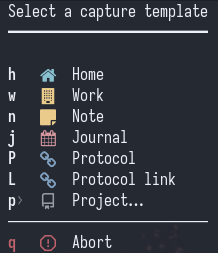
\includegraphics[width=0.58\textwidth]{capture.png}
\end{center}
\note{
\tiny

One of the more powerful use-cases for org-mode is (shockingly) organisation. The first stages of planning are capturing ideas. As you're coding or planning, you have a brainwave and you need to quickly jot something down to revisit later.

This is where org-capture comes in, and lets you define extensible templates (my complicated example borrowed from tecosaur) to let you quickly pop open a note to be saved to a pre-defined org file, or even ``refile'' to another file.

These templates let you pre-populate things like the date if say you're creating a task, or the line in the file you're at when you invoke if you're recording a project note.}
\end{frame}
\section{Agenda}
\label{sec:org7c12c97}
\begin{frame}[label={sec:org783eebf},fragile]{Schedule tasks}
 \bigskip
\begin{Code}
\begin{Verbatim}
\color{EFD}\textcolor[HTML]{2E3440}{*}\textcolor[HTML]{a0522d}{*} \textcolor[HTML]{A3BE8C}{\textbf{TODO}} \textcolor[HTML]{a0522d}{Finish this Safari}
\textcolor[HTML]{78808f}{SCHEDULED:} \textcolor[HTML]{EBCB8B}{<2023-10-11 Wed>}
\textcolor[HTML]{78808f}{DEADLINE:} \textcolor[HTML]{EBCB8B}{<2023-10-11 Wed>}
\end{Verbatim}
\end{Code}
\note{
\tiny

So we've touched on tasks briefly, but when we say task we very simply mean a ``heading'' that has a state. Once it has a state keyword, it is a valid task that can be used as part of the agenda. You can also link dates to that task, and this status will show up in the associated agenda views and also lets you ask questions of your tasks; say ``Which tasks are scheduled to be done in the next 4 days?'' or ``What deadlines do I have next week?''.}
\end{frame}
\begin{frame}[label={sec:org78917a7},fragile]{Repeating tasks/habits}
 \bigskip
\begin{Code}
\begin{Verbatim}
\color{EFD}\textcolor[HTML]{2E3440}{*}\textcolor[HTML]{a0522d}{*} \textcolor[HTML]{A3BE8C}{\textbf{TODO}} \textcolor[HTML]{a0522d}{Mention how useful org-mode is}
\textcolor[HTML]{78808f}{DEADLINE:} \textcolor[HTML]{EBCB8B}{<2023-10-11 Wed +1h>}
\end{Verbatim}
\end{Code}
\note{
\tiny

Similar to scheduling one-off tasks, you can also mark a task as ``repeated'' by adding a repeater at the end (in this case I mention how useful org-mode is every hour). When viewing these in an agenda view, they would show up differently and let you track and record each ``instance'' of completion, say if you were tracking a habit instead.

There's a useful tutorial \href{https://orgmode.org/worg/org-tutorials/tracking-habits.html}{here} on habit tracking.

See more on repeated tasks in the \href{https://orgmode.org/manual/Repeated-tasks.html}{manual}.}
\end{frame}
\begin{frame}[label={sec:orgfd9a0cd},fragile]{Task status/reason}
 \bigskip
\begin{Code}
\begin{Verbatim}
\color{EFD}\textcolor[HTML]{2E3440}{*}\textcolor[HTML]{a0522d}{*} \textcolor[HTML]{A3BE8C}{\textbf{TODO}} \textcolor[HTML]{a0522d}{Finish this section}
\textcolor[HTML]{2E3440}{*}\textcolor[HTML]{a0522d}{*} \textcolor[HTML]{A3BE8C}{\textbf{INPROG}} \textcolor[HTML]{a0522d}{Present my Safari}
\textcolor[HTML]{2E3440}{*}\textcolor[HTML]{a0522d}{*} \textcolor[HTML]{4C566A}{\textbf{DONE}} \textcolor[HTML]{4C566A}{Create jokes for the viewers}
\end{Verbatim}
\end{Code}

\begin{Code}
\begin{Verbatim}
\color{EFD}\EFrda{(}\EFo{cdar} \EFv{org-todo-keywords}\EFrda{)}
\end{Verbatim}
\end{Code}

\begin{Code}
\begin{Verbatim}
\color{EFD}\EFrda{(}\EFs{"}\textcolor[HTML]{ff8e00}{\textbf{TODO}}\EFs{(t)"} \EFs{"INPROG(i)"} \EFs{"PROJ(p)"} \EFs{"STORY(s)"} \EFs{"WAIT(w@/!)"} \EFs{"|"} \EFs{"DONE(d@/!)"}
 \EFs{"KILL(k@/!)"}\EFrda{)}
\end{Verbatim}
\end{Code}
\note{
\tiny

The status of a task comes from a defined set of keywords, the above showing what's defined for me. In short, everything before the \texttt{|} value defines tasks that have some kind of ``action'' applied to them, in order to advance it to the next state. The last two, \texttt{DONE} and \texttt{KILL} and ``end points'' for a task, no further action is needed here.

The other symbols denote things like whether or not you should be prompted to add an entry to the \texttt{LOGBOOK} drawer.

For further info, see the docstring for \texttt{org-todo-keywords}.}
\end{frame}
\section{Agenda Demo}
\label{sec:orge2ac581}
\note{
\tiny

Showcase creating task from capture, logbook, date picker, cycling through states}
\section{Babel}
\label{sec:orgc358cf1}
\begin{frame}[label={sec:orgd2e434e},fragile]{So what's with all these code blocks?}
 \bigskip
\begin{Code}
\begin{Verbatim}
\color{EFD}\EFobb{\#+begin\_src emacs-lisp :exports both}
\textcolor[HTML]{707183}{(}\textcolor[HTML]{008b8b}{list} \textcolor[HTML]{7388d6}{(}\textcolor[HTML]{008b8b}{list} \textcolor[HTML]{8b2252}{"Header"} \textcolor[HTML]{8b2252}{"Value"}\textcolor[HTML]{7388d6}{)}
      \textcolor[HTML]{7388d6}{(}\textcolor[HTML]{008b8b}{list} \textcolor[HTML]{8b2252}{"Date"} \textcolor[HTML]{909183}{(}\textcolor[HTML]{008b8b}{current-time-string}\textcolor[HTML]{909183}{)}\textcolor[HTML]{7388d6}{)}
      \textcolor[HTML]{7388d6}{(}\textcolor[HTML]{008b8b}{list} \textcolor[HTML]{8b2252}{"It's just data"} \textcolor[HTML]{8b2252}{"\$x=\char92{}\char92{}frac\{-b\char92{}\char92{}pm\char92{}\char92{}sqrt\{b\char94{}2-4ac\}\}\{2a\}\$"}\textcolor[HTML]{7388d6}{)}\textcolor[HTML]{707183}{)}
\EFobe{\#+end\_src}
\end{Verbatim}
\end{Code}

\begin{Code}
\begin{Verbatim}
\color{EFD}\EFrda{(}\EFo{list} \EFrdb{(}\EFo{list} \EFs{"Header"} \EFs{"Value"}\EFrdb{)}
      \EFrdb{(}\EFo{list} \EFs{"Date"} \EFrdc{(}\EFo{current-time-string}\EFrdc{)}\EFrdb{)}
      \EFrdb{(}\EFo{list} \EFs{"It's just data"} \EFs{"\$x=\char92{}\char92{}frac\{-b\char92{}\char92{}pm\char92{}\char92{}sqrt\{b\char94{}2-4ac\}\}\{2a\}\$"}\EFrdb{)}\EFrda{)}
\end{Verbatim}
\end{Code}

\begin{center}
\begin{tabular}{ll}
\toprule
Header & Value\\[0pt]
Date & Wed Oct 11 13:54:40 2023\\[0pt]
It's just data & \(x=\frac{-b\pm\sqrt{b^2-4ac}}{2a}\)\\[0pt]
\bottomrule
\end{tabular}
\end{center}
\end{frame}
\note{
\tiny

\emph{Finally} we come to these code blocks; these are part of what's called Org-Babel. Named after the biblical tale that told of a race of humans that spoke the same language trying to build a tower to the heavens. Yanweh, a deity, observed and punished the humans by making them all speak different languages; making constructing the tower impossible. He then scattered the humans, and that apparently is where the origin of everyone speaking different languages come from.

Unlike the story though, we can leverage multiple languages to our advantage. These code blocks can be executed, with many \href{https://orgmode.org/worg/org-contrib/babel/languages/index.html}{languages} having an org-babel extension (shortened to ob) instructing babel how to run and interpret results from various languages.

Here we have an example of a simple code block, also showing how you pass options to the execution of said block. Here, we're instructing org-babel to export both the code and the results when the document is exported (more in the next section). And because the result is a cons list, babel by default renders the output as a table, which has been exported above in latex (including the quadratic formula)}
\begin{frame}[label={sec:org833bb78},fragile]{Notebooks}
 First we define \emph{the} most useful function we're ever likely to use

\begin{Code}
\begin{Verbatim}
\color{EFD}\EFrda{(}\EFk{defn} \EFf{super-cool-fn} \EFrdb{[}\EFrdb{]}
  \EFhn{42}\EFrda{)}
\end{Verbatim}
\end{Code}

\begin{verbatim}
#'user/super-cool-fn
\end{verbatim}


Then; we execute it. There might be a race condition here, I didn't verify if the channel was closed so the output might come in order of out.

\begin{Code}
\begin{Verbatim}
\color{EFD}\EFrda{(}super-cool-fn\EFrda{)}
\end{Verbatim}
\end{Code}

\begin{verbatim}
42
\end{verbatim}
\note{
\tiny

A good use-case for this is the idea of a ``literate notebook'', with code sections interspersed with prose. Here we have a small sample of what could be one such notebook, these code blocks are run inside of the same ``session'' (what a session is differs from executor-to-executor, but here it's a cider REPL) meaning that each code block has access to the same code as any other block marked in that session.

If you're reading this after the fact, check the properties drawer under the heading.}
\end{frame}
\begin{frame}[label={sec:org2007ce1},fragile]{Piping results}
 \tiny

\begin{Code}
\begin{Verbatim}
\color{EFD}\EFk{import} hashlib, zlib, os
\EFv{string\_to\_hash} = \EFs{'Hello from Org-Mode'}
\EFv{header} = \EFs{"blob "} + \EFb{str}(\EFb{len}(string\_to\_hash)) + \EFs{"}\EFo{\char92{}0}\EFs{"}
\EFv{blob} = (header + string\_to\_hash).encode(\EFs{'utf8'})
\EFv{sha} = hashlib.sha1(blob).hexdigest()
\EFv{git\_object} = f\EFs{".git/objects/}\{sha[:2]\}\EFs{/}\{sha[2:]\}\EFs{"}
os.makedirs(os.path.dirname(git\_object), exist\_ok=\EFo{True})
\EFk{with} \EFb{open}(git\_object, \EFs{'wb'}) \EFk{as} f:
    f.write(zlib.compress(blob))

\EFk{return} f\EFs{"Wrote:} \{git\_object\}\EFs{"}
\end{Verbatim}
\end{Code}

\begin{verbatim}
Wrote: .git/objects/fc/86439179b93382f976c577895ed72011f766c6
\end{verbatim}


\begin{Code}
\begin{Verbatim}
\color{EFD}\EFt{git} cat-file -p \EFs{'fc86'}
\end{Verbatim}
\end{Code}

\begin{verbatim}
Hello from Org-Mode
\end{verbatim}


\href{https://www.youtube.com/watch?v=0g9BcZvQbXU}{Source}
\note{
\tiny

Here we have what looks like a simple snippet of python (from another talk I've done on Git Fundamentals), but when we look at the code behind it shortly you'll see that there's couple of useful features here; piping results to other blocks and what's referred to as ``noweb'' syntax letting you refer to the results of other code blocks directly.

The hash object being written here is \emph{actually} being written and retrieved, and the value of ``I am a file'' is coming from another code block. By simply parametrizing these blocks, you can easily create a rich set of demos that are very easy to modify.}
\end{frame}
\section{Export}
\label{sec:org4ef24e5}
\begin{frame}[label={sec:org08fa610}]{How did I make this presentation?}
\begin{center}
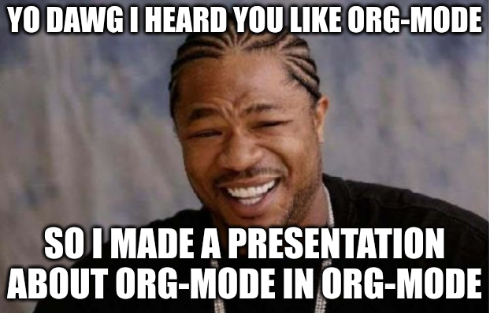
\includegraphics[width=.9\linewidth]{dawg.png}
\end{center}
\note{
\tiny

And now we finally get to export. \emph{Another} fantastic feature of org-mode that lets you take an org document and run it through an org-exporter (shorted to ox, like org-babel and ob) to produce some other format.

The most common of which are \LaTeX (which is how this presentation has been created) and HTML, for example \href{https://elken.github.io/doom/}{my Doom Emacs config}.

This is done through a number of backends, one such being pandoc; instantly giving you access to a large variety of output formats.

As you've seen from previous slides, any raw \LaTeX code gets translated verbatim; the same applies to any HTML or any other format specs}
\end{frame}
\section{Export Demo}
\label{sec:orgb2bdf80}
\note{
\tiny

Showcase the inner workings of the git slide, adjust some of the values and re-export, the many formats available ootb with Doom, run through the document behind the presentation}
\section{Advanced Use-Cases}
\label{sec:org853fdee}
\begin{frame}[label={sec:orgdb4666c},fragile]{Literate configuration}
 \begin{Code}
\begin{Verbatim}
\color{EFD}\textcolor[HTML]{2E3440}{*}\textcolor[HTML]{a0522d}{*} \textcolor[HTML]{a0522d}{My super cool Emacs config}
\EFobb{\#+begin\_src emacs-lisp :tangle init.el}
\textcolor[HTML]{707183}{(}\textcolor[HTML]{008b8b}{message} \textcolor[HTML]{8b2252}{"Emacs Started!"}\textcolor[HTML]{707183}{)}
\EFobe{\#+end\_src}
\end{Verbatim}
\end{Code}

\begin{Code}
\begin{Verbatim}
\color{EFD}\EFrda{(}\EFk{let*} \EFrdb{(}\EFrdc{(}\EFv{default-directory} \EFv{user-emacs-directory}\EFrdc{)}
       \EFrdc{(}changed-at \EFrdd{(}\EFf{file-attribute-modification-time} \EFrda{(}\EFo{file-attributes} \EFs{"config.org"}\EFrda{)}\EFrdd{)}\EFrdc{)}\EFrdb{)}
  \EFrdb{(}\EFo{require} \EFhq{'}\EFo{org-macs}\EFrdb{)}
  \EFrdb{(}\EFk{unless} \EFrdc{(}\EFo{org-file-newer-than-p} \EFs{"init.el"} changed-at\EFrdc{)}
    \EFrdc{(}\EFo{require} \EFhq{'}\EFo{ob-tangle}\EFrdc{)}
    \EFrdc{(}\EFo{org-babel-tangle-file} \EFs{"config.org"} \EFs{"init.el"} \EFs{"emacs-lisp"}\EFrdc{)}\EFrdb{)}
  \EFrdb{(}\EFo{load-file} \EFs{"init.el"}\EFrdb{)}\EFrda{)}
\end{Verbatim}
\end{Code}
\note{
\tiny

Many Emacs users (myself included) use what's referred to a ``literate configuration'', which similar to the notebooks idea is a configuration file exported from code blocks interspersed with regular prose.

This allows you to have a very neat configuration that will be nicely readable in Emacs, in some code forge like Github or even better exported to a format like PDF (via \LaTeX) or HTML.

It also leads nicely into our next use-case, which we've briefly touched on before}
\end{frame}
\begin{frame}[label={sec:org31a93b5},fragile]{Compile-time dynamic content}
 \begin{Code}
\begin{Verbatim}
\color{EFD}\textcolor[HTML]{78808f}{\#+NAME: keyboard-device-file}
\EFobb{\#+begin\_src shell}
\textcolor[HTML]{228b22}{find} \EFob{/dev/input/by-}\textcolor[HTML]{707183}{\{}\EFob{path,id}\textcolor[HTML]{707183}{\}} \EFob{-name} \textcolor[HTML]{8b2252}{'*-kbd'} \EFob{| head -n} \textcolor[HTML]{008b8b}{\textbf{1}} \EFob{| tr -d} \textcolor[HTML]{8b2252}{"\char92{}n"}
\EFobe{\#+end\_src}

\EFobb{\#+begin\_src kbd :tangle kmonad.kbd :noweb yes}
\EFob{(defcfg}
  \EFob{input (device-file "<<keyboard-device-file()>>")}
  \EFob{output (uinput-sink "My KMonad output")}
  \EFob{fallthrough true)}

\EFob{...}
\EFobe{\#+end\_src}
\end{Verbatim}
\end{Code}

Courtesy of \href{https://github.com/ambirdsall/dots/blob/master/.config/kmonad/config.org}{ambirdsall}.
\note{
\tiny

We've touched on something called ``noweb'' before, but here it is in with a great use-case.

\texttt{kmonad} is a tool for creating bespoke layouts using a lisp-like language. Here, it needs the keyboard device file; but that's never guaranteed to be the same across keyboards, systems, etc. So instead of updating the file constantly, here we can use the result of the now named block \texttt{keyboard-device-file} and add it in the below file in the chevrons with empty parens (since these blocks can also take arguments).

We also see the \texttt{tangle} execution option, which lets us redirect the output of the block to a file instead.

This can be useful for all manner of things, say you prefer a particular theme across all your devices. You can define a table with all the colours in it, and use that in every other place you need to ``tangle'' other config files. Update the table, and all your other files will be updated.

This is also a great option for handling secrets, you can have a code block to return a result from \texttt{pass} or equivalent password manager and have that secret be tangled into any files that need them.}
\end{frame}
\begin{frame}[label={sec:org3531c26},fragile]{Export snippets}
 \begin{Code}
\begin{Verbatim}
\color{EFD}\textcolor[HTML]{78808f}{:header-args:snippet:} \textcolor[HTML]{78808f}{:mkdirp yes :tangle (expand-file-name (downcase (car (last (org-get-outline-path t)))) (expand-file-name (downcase (car (last (butlast (org-get-outline-path t))))) "snippets"))}
\end{Verbatim}
\end{Code}

\begin{Code}
\begin{Verbatim}
\color{EFD}tree \char126{}/.config/doom/snippets
\end{Verbatim}
\end{Code}

\begin{Code}
\begin{Verbatim}
\color{EFD}/home/lkn/.config/doom/snippets
├── clojure-ts-mode
│   └── \_\_bb.edn
├── org-mode
│   └── \_\_
└── slack-message-compose-buffer-mode
    └── standup

\EFhn{4} directories, \EFhn{3} files
\end{Verbatim}
\end{Code}
\note{
\tiny

Here we have one from my personal literate configuration, using the structure of org-mode to create yasnippet snippets. Using \texttt{tangle}, we're simply telling org-mode the file should be the second-to-last header the code block is under, followed by the last header; which in my config is the mode-name followed by the file name (the format yasnippet expects)

There's other code that goes with it, I've made a small guide on setting this up \href{https://discourse.doomemacs.org/t/org-tips-and-tricks-thread/2718/4}{here}.}
\end{frame}
\begin{frame}[label={sec:org58ea37f},fragile]{Static site generation}
 \begin{Code}
\begin{Verbatim}
\color{EFD}\EFrda{(}\EFk{setq} \EFv{org-publish-project-alist}
      \EFhq{`}\EFrdb{(}\EFrdc{(}\EFs{"files"}
         \EFb{:base-directory} ,\EFv{doom-user-dir}
         \EFb{:base-extension} \EFs{"org"}
         \EFb{:publishing-directory} \EFs{"out"}
         \EFb{:exclude} \EFs{"README.org"}
         \EFb{:publishing-function} org-html-publish-to-html
         \EFb{:completion-function} +org-publish-rename
         \EFb{:with-creator} t
         \EFb{:section-numbers} nil\EFrdc{)}

        \EFrdc{(}\EFs{"site"} \EFb{:components} \EFrdd{(}\EFs{"files"}\EFrdd{)}\EFrdc{)}\EFrdb{)}\EFrda{)}

\EFrda{(}\EFo{org-publish-project} \EFs{"site"} t\EFrda{)}
\end{Verbatim}
\end{Code}
\note{
\tiny

Implied by the idea of being able to export a file, it's also possible to create a ``publish project'' of various files and merge them together to create a published output.

Here is a simplified snippet from the script used to export my own literate config. You can define many components for various files, for example static content you have to run through a pre-processor or images you have to compress first.

These are then called by \texttt{org-publish-project} which produces the output you see \href{https://elken.github.io/doom/}{here}.}
\end{frame}
\section{Closing}
\label{sec:org6403674}
\begin{frame}[label={sec:orgecd58fc}]{Wider ecosystem}
\begin{itemize}
\item \href{https://github.com/org-roam/org-roam}{org-roam}
\item \href{https://github.com/tecosaur/ox-chameleon}{ox-chameleon}
\item \href{https://github.com/alf/ob-restclient.el}{ob-restclient}
\item \href{https://github.com/dengste/org-caldav/}{org-caldav}
\item \href{https://github.com/nobiot/org-transclusion/}{org-transclusion}
\item \href{https://gohugo.io/}{hugo} and \href{https://ox-hugo.scripter.co/doc/quick-start/}{ox-hugo}
\end{itemize}
\note{
\tiny

Nearly there now, here's just a snippet of some of my favourite packages in the wider org ecosystem.

org-roam I'm sure many of you are at least somewhat familiar with, it's an implementation of Roam Research's tool for managing personal information. What's here is worthy of a Safari on its own, but it's worth looking into

ox-chameleon is the fantastic package being used here to have the presentation use my theme of choice, Nord, all over. The package also supports HTML exports, and there's a PR I've had ongoing to include the extra niceties found on my exported config. You'll likely have noticed some inconsistencies with how some code blocks are coloured, there's a bug in ox-chameleon that's not yet resolved causing it to default to the base colour scheme rather than mine..

ob-restclient is an org-babel extension for restclient.el allowing you to create a notebook for a REST API (there's one for GraphQL too). This is great for producing a self-annotating README for an API or service

org-caldav is one I've moved away from, but in essence it lets you manage calendar events through caldav using org-mode. Integrating with G suite, Office 365 etc you can manage all your events through Emacs, link to events easily, refer to them from emails, etc

org-transclusion is a simple package which lets you insert a copy of a file's content using a regular file link. Great for creating nested documents, worth checking out the README if you're interested

And lastly I've included Hugo here because it indirectly supports org-mode posts (with another package inbetween) and is commonly how people manage blogs using posts and pages written in org-mode

I've barely scratched the surface both on what's included as part of Emacs and what's available wider, so I encourage you to read through the manual and explore what's out there.}
\end{frame}
\section{Any questions?}
\label{sec:org9ac156e}
\end{document}